%!TEX root = /Users/markelikalderon/Documents/Git/formwithoutmatter/aristotle.tex
\chapter{The Generation of the Hues} % (fold)
\label{cha:the_generation_of_the_hues}

\section{Aristotle's Three Models} % (fold)
\label{sec:aristotle_s_three_models}

That white and black, or, better yet, light and dark, are the primary colors, the colors in terms of which all other colors can be explained, is an ancient doctrine arguably of Homeric roots. As presented by Parmenides, in the Way of Mortal Opinion, Fire and Night are cosmic principles standing in opposition whose attributes consists of sensible qualities arrayed in pairs of contraries. Brightness and darkness as they appear in sensory experience are one such pair of attributes. Brightness is an attribute of Fire just as darkness is an attribute of Night, and the opposition of these cosmic principles is partly manifest in this pair of sensible qualities being contraries. Empedocles shares Parmenides' conception of light and dark as contrary sensible qualities. According to Parmenides, brightness is an attribute of Fire. It has others. Fire must then be independent of brightness, in some appropriate sense. In seeing the sun burning bright, what one sees is a manifestation of the operation of the cosmic principle of Fire. It is the activity of the fiery principle that explains the brightness of distal objects. Empedocles also takes over from Parmenides this explanatory priority. White or light is explained in terms of the element of fire composing the effluences emitted from distal objects themselves composed of a preponderance of fire. In contrast, black or dark is explained in terms of the element of water composing the effluences emitted from distal objects themselves composed of a preponderance of water. 

Empedocles, however, makes two important contributions (at least on my partial and selective account of this ancient tradition). First, not only are the sensible qualities, light and dark, conceived as contraries, but, like hot and cold, as endpoints of an ordered range of sensible qualities. The chromatic hues are the sensible qualities intermediate between the extremes of light and dark. Second, on Parmenides' account, the chromatic hues that objects appear to have, as well as ``the whole world of sense'', are the result of ``blending'' Fire and Night (Plutarch, \emph{Adversus Colotem} 1114\( ^{b-c} \)). However, the Way of Mortal Opinion, at least in the fragmentary state in which it has come down to us, does not elaborate how the blending of Fire and Night results in the appearance of chromatic hues in our sensory experience. Empedocles second contribution is that it is the \emph{proportion} or \emph{ratio} of Fire and Night, or in terms of his own cosmology, the ``roots'' or elements fire and water, that gives rise to the appearance of chromatic hues in our sensory experience of the natural environment. It is plausible that neither contribution is original to Empedocles. Thus, for example, \citet{Gladstone:1858fk} discerns the former in the Homeric color scheme. Moreover, the emphasis on the proportion or ratio of Fire and Night is arguably implicit in the Parmenidean fragments: Justice governs the sensible world presumably by governing the changing proportions of Fire and Night in the cosmic mixture.

Much of Empedocles work is an attempt to reconcile putative Parmenidean insights with the way things appear in our sensory experience. Empedocles accepts the central lesson of the Way of Mortal Opinion that one must posit a plurality of principles in opposition if one is to accommodate the plurality and opposition encountered in sensory experience and so abandon's Parminedes' monism (though his ``roots'' or elements are in effect Parmenidean beings despite their plurality since they are insusceptible to alteration, growth, or decay). Aristotle too wishes to save the phenomena while preserving the insights of his predecessors, Parmenides and Empedocles prominent among them. Indeed he is the great defender of the manifest image in the classical world. Moreover, Aristotle takes over from Empedocles the general idea that the chromatic hues result from the proportion or ratio of light and dark. Aristotle provides an extended discussion of how these ratios might be implemented. First, he offers three accounts, in terms of (1) juxtaposition, (2) overlap, and (3) mixture, opting for the third. Second, he provides an account of what the chromatic proportions or ratios are, and makes some important related claims about the ordering of sensible qualities between the extremes of light and dark.

\subsection{Juxtaposition} % (fold)
\label{sub:juxtaposition}

Aristotle presents the first account as follows:
\begin{quote}
	We must now treat of the other colours, reviewing the several ways in which they can come about. It is conceivable that the white and the black should be juxtaposed in quantities so minute that either separately would be invisible, though the joint product would be visible; and that they should thus have the other colours for resultants. Their product could, at all events, appear neither white nor black; and, as it must have some colour, and can have neither of these, this colour must be of a mixed character---in fact, a species of colour different from either. Such, then, is a possible way of conceiving the existence of a plurality of colours besides the white and black; (Aristotle, \emph{De Sensu} \textsc{iii} 439\( ^{b} \)18--28; Beare in \citealt[8]{Barnes:1984uq})
\end{quote}
Aristotle asks us to imagine a visible compound composed of white and black parts, themselves too small to be visible. Since the compound is visible it must have some color. Since the white and black parts are too small to be visible, the color of the compound could not be either of these. So the compound must have some other kind of color. And it is the proportion of white and black components that determines the given chromatic hue. The remainder of the passage develops this suggestion. 

Familiarity with pointillism and color halftone printing can obscure for us the real achievement in Aristotle's entertaining the possibility that the color of a compound can differ from the color of its parts. Pointillist paintings and color halftone prints have minute parts that differ in color from the painting or print as a whole at least when viewed from a suitable distance. Michel Eugène Chevreul, a French chemist appointed by Louis \textsc{xvii} as the director of the dye department of Manufacture Royale des Gobelins, upon receiving complaints that the black dyes they produced looked different when used alongside blue dye, investigated the matter and discovered the phenomena of simultaneous color contrast---that the appearance of a color can vary as the color of the surrounding scene varies. \citet{Chevreul:1855kx} reported his findings in his book, \emph{The Principles of Harmony and Contrast of Colours and Their Application to the Arts}, a book that influenced the work of the French painter Georges-Pierre Seurat. Fascinated by the appearance of a color being influenced by adjacent colors, Seurat eventually paints the pointillist masterpiece, “Un dimanche après-midi à l'Île de la Grande Jatte” in 1884--6 (see figure~\ref{fig:jatte}). Using only primary unblended pigments, including the newly available zinc yellow, these were distributed in small dots across the surface of the canvas giving rise to the appearance, at an appropriate distance, of a differently colored scene of Parisian suburbanites relaxing by the river Seine. The analogy is imperfect, however, in that the minute parts of the painting and print are merely too small to be seen from a suitable distance, where as the white and black parts of Aristotle's compound are too small to be seen at any distance.

\begin{figure}[htbp]
    \centering
        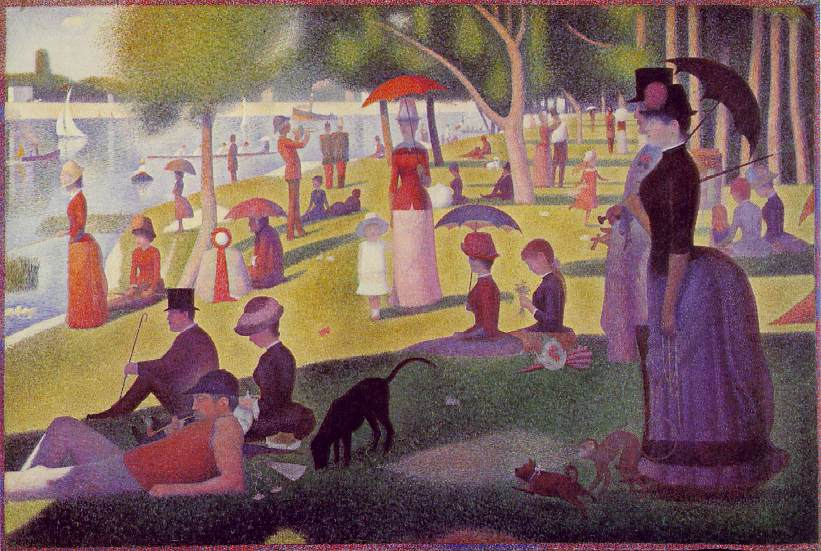
\includegraphics[scale=0.70]{graphics/jatte.jpg}
    \caption{Georges-Pierre Seurat, “Un dimanche après-midi à l'Île de la Grande Jatte”}
    \label{fig:jatte}
\end{figure}


Notice that on the proposed account color is not dissective in something like Goodman's \citeyearpar[53]{Goodman:1951ww} sense of the term. A property \( p \) is \emph{dissective} just in case if \( p \) is instantiated by a whole, \( p \) is instantiated by each of its parts. (Dissectivity is a broader notion than being homoeomerous since the latter is restricted to substance kinds, \emph{De Generatione et Corruptione} \textsc{i} 10 328\( ^{a} \)6ff.) So if color were dissective, then the color of the whole would be the color of its parts. The color of a whole may be a function of the color of its parts, a point on which Aristotle and Goodman agree, but that does not mean that the function will determine color to be dissective:
\begin{quote}
	Different perceptible parts of any object may be differently colored even if the object itself is uniform and unvarying in color. This is no more paradoxical than the fact that a single object contains spatiotemporally different parts. As the self-identical object is a function of its parts, so the single unchanging color of the object is a function of the colors of its parts. The nature and interrelation of the lesser elements that make up the whole determine what kind of thing the whole is: the kind and arrangement of the colors exhibited by these various parts determine what color the whole is said to have. \citep[130]{Goodman:1951ww}
\end{quote}

On the present account, we can see the blue of the sea even though we fail to see its white and black parts since they are too are too small to be seen. A consequence of the juxtaposition model is that it is possible to see the color of a whole without seeing the distinct colors of the parts that compose it. That thought, however, is only intelligible set against a background conception of perception as providing a \emph{partial} perspective on the natural environment. The partiality of perception has recently been defended by \citet{Hilbert:1987jq}, but it has ancient roots as well---arguably, Heraclitus is an advocate \citep[see][]{Burnyeat:1979mv,Kalderon:2006tg}. Not only is perception partial in the sense that there are properties of an object not perceptually available (objects may have unobservable aspects), not only is perception partial in the sense that some sensible qualities of an object may be occluded from view (the backs of objects are colored as well), but perception is also partial in the sense there are sensible qualities of an object that are not determined by a given perception. If one can see the color of a whole while failing to see the distinct colors of its parts, then one can see some if not all of an object's chromatic features. One sees the blue of the sea but not that it is partly white and partly black. This is only possible if perception is partial in something like the sense described above. 

I am uncertain whether Aristotle genuinely subscribes to some version of this doctrine. While it is a commitment of the juxtaposition model, this is a model that he rejects. However, while a commitment of the juxtaposition model, the partiality of perception is not itself committed to that model. Doubts about the juxtaposition model need not undermine the partiality of perception. Earlier we registered a disanalogy between the juxtaposition model, on the one hand, and pointillism and color halftone printing, on the other. While the latter involves parts too small to be seen from a certain distance, the former involves parts too small to be seen at any distance. The partiality of perception is manifest in viewing the color of a pointillist painting---one sees the color of the whole without seeing the colors of its parts. Moreover, this is consistent with the Aristotelian denial of invisible magnitudes. So even if there are no parts too small to be seen from any distance, this would not, by itself, cast doubt on the partiality of perception. If Aristotle does indeed retain some, perhaps attenuated, version of this doctrine, this would go some way towards explaining his sanguine attitude towards putative cases of conflicting appearances \citep[on how the partiality of perception can help dissipate some appearances of conflict see][]{Kalderon:2006tg}.

Aristotle rejects the juxtaposition model partly on the grounds that it posits colored objects too small to be seen (\emph{De Sensu} \textsc{iii} 440\( ^{a} \)21--25). Such parts would have magnitude and yet would be invisible. But, according to Aristotle, there are no invisible magnitudes. Every magnitude is visible from some distance. And while the color of some wholes dissolve upon closer inspection, such as Seurat's masterpiece (figure~\ref{fig:jatte}) or the color halftone printing of the Marvel Comics of my childhood (figure~\ref{fig:wolverine}), not all do. There are some surfaces that retain their color no matter how closely we look (compare \emph{De Sensu} \textsc{iii} 440\( ^{b} \)16--18 discussed further in the next section~\ref{sub:overlap}). So the juxtaposition model is implausibly revised to claim instead that the colors of compounds are determined by the juxtaposition of minute white and black parts that are normally not visible. It is open to ready empirical disconfirmation when we fail to discover these black and white parts despite our best efforts.

\begin{figure}[htbp]
    \centering
        
\includegraphics[scale=5]{graphics/wolverine.jpg}
    \caption{Detail of Wolverine from \emph{X-Men}, 1963}
    \label{fig:wolverine}
\end{figure}

In his initial presentation of the juxtaposition model, Aristotle considers a case involving the spatial juxtaposition of white and black parts. He also considers a variant of this model, where the white and black things are not spatially juxtaposed but are instead temporally juxtaposed. Set in the context of the theory of effluences, the idea is that the temporal juxtaposition of the white and black effluences assimilated by the organ of sight gives rise to a chromatic appearance. Just as spatial inhomogeneities of the compound body composed of white and black parts determines a proportion or ratio of light and dark characteristic of say, blue, it is the temporal inhomogeneities of the assimilated effluences---now white, now black---that determines a proportion of light and dark characteristic of blue. In this regard, the temporal variation of the juxtaposition model is analogous to the way in which Benham's spinning disk can give rise to chromatic appearances.

The temporal variant of the juxtaposition model faces a parallel problem as the spatial variant. Just as the spatial variant of the juxtaposition model was committed to imperceptible spatial magnitudes, the temporal variant is committed to imperceptible temporal magnitudes and for much the same reason:
\begin{quote}
	If we accept the hypothesis of juxtaposition, we must assume not only invisible magnitude, but also imperceptible time, in order that the arrival of the movements may be unperceived, and that the colour may appear to be one because they seem to be simultaneous. (Aristotle, \emph{De Sensu} \textsc{iii} 440\( ^{a} \)20--25; Beare in \citealt[9]{Barnes:1984uq})
\end{quote}
Consider alternating assimilations of white and black effluences by the organ of sight occurring in a certain temporal ratio. The pattern of alternating assimilations is perceptible. The pattern at least determines the experience of a chromatic hue. But our experience of a color of a particular is not the experience of a succession of light and dark. So the assimilation of white and black effluences must occur too quickly to be individually perceptible. However, if temporally juxtaposed in the right proportion, the temporal compound, the pattern of alternating assimilations, would be perceptible.  Indeed, it would be the perception of the chromatic hue. Unfortunately, just as Aristotle rejects imperceptible spatial magnitudes, he also rejects imperceptible temporal magnitudes and with it the temporal variant of the juxtaposition model.

% subsection juxtaposition (end)

\subsection{Overlap} % (fold)
\label{sub:overlap}
On the first model, chromatic hues are determined by a proportion of light and dark that arises from light and dark objects being temporally or spatially juxtaposed. The second model that Aristotle considers works not by means of juxtaposition, but by means of overlap:
\begin{quote}
	Another is that the black and white appear the one through the medium of the other, giving an effect like that sometimes produced by painters overlaying a less vivid upon a more vivid colour, as when they desire to represent an object appearing under water or enveloped in a haze, and like that produced by the sun, which in itself appears white, but takes a crimson hue when beheld through a fog or a cloud of smoke. On this hypothesis, too, a variety of colours may be conceived to arise in the same way as that already described; for between those at the surface and those underneath a definite ratio might sometimes exist; in other cases they might stand in no determinate ratio. (Aristotle, \emph{De Sensu} \textsc{iii} 440\( ^{a} \)7--15; Beare in \citealt[8--9]{Barnes:1984uq})
\end{quote}
Perhaps colors are not so much juxtaposed as they are overlapping. The overlapping colors, however, are importantly perceptually penetrable at least to some degree---they appear through one another. Suppose one color overlays another color. If the overlaying color is perceptually impenetrable, if it determines a visual boundary through which nothing further could appear, the underlying color would be occluded, and this would not be a method of color combination since only the overlaying color could be seen. If overlaying and underlying colors are genuinely combined by overlap, then at least the overlaying color must be perceptually penetrable at least to some degree. Moreover, it cannot be perfectly transparent. If the overlaying color were perfectly transparent, it would be wholly receptive of the underlying color, and, again, this would not be a method of color combination since only the underlying color could be seen. For the overlap model to work, at least the overlaying color must be imperfectly transparent. The overlaying color's contribution to the resulting chromatic appearance consists, in part, in the visual resistance it offers:
\begin{quote}
	\ldots\ the stimulatory process produced in the medium by the upper colour, when this is itself unaffected, will be different in kind from that produced by it when affected by the underlying colour. Hence it presents itself as a different colour, i.e. as one which is neither white nor black. (Aristotle, \emph{De Sensu} \textsc{iii} 440\( ^{a} \)24--28; Beare in \citealt[9]{Barnes:1984uq})
\end{quote}
Moreover, the ratio of the overlapping colors that results in the novel color is partly determined by the degree of visual resistance offered by the imperfectly transparent overlaying color.

The painting analogy is arguably a deliberate echo of Empedocles (\textsc{dk} 31\textsc{b}23). As in the Emepedoclean fragment, the method of color combination deployed by the painters is overlaying semi-transparent colored washes---the method that Plutarch attributes to Apollodorus and is characteristic of Greek four-color painting more generally. Aristotle's choice of depicted content further emphasizes this: He draws our attention to how a painter might depict something appearing through water or mist by overlaying a wash of some appropriate color. Here perceptually penetrable washes of pigment are the means of representing something that is itself perceptually penetrable---the water or mist through which the object appears. He draws our attention to the imperfectly transparent subject matter as a way of emphasizing the imperfectly transparent means of representing that subject matter. The painting analogy thus further confirms that at least the overlaying color must be imperfectly transparent.

The sun seen through a fog or cloud of smoke is Aristotle's second analogy. The sun is white, and the smoke is black. And yet when the cloud of smoke is superimposed over the sun, it gives rise to a crimson appearance. If the black of the smoke were perceptually impenetrable, if it determined a visual boundary through which nothing further could appear, then the white of the sun would have been occluded by the black of the smoke, and a method of color combination could not be understood on this analogy since only the overlaying color could be seen. If on the other hand, the smoke were perfectly transparent, it would be wholly receptive to the white of the sun and, again, a method of color combination could not be understood on this analogy since only the underlying color could be seen. For the analogy to work, the smoke must be imperfectly transparent, the blackness of the smoke contributes to the resulting chromatic appearance, in part, by the visual resistance it offers. Though it remains receptive of the white of the sun, otherwise it would be opaque, the darkness of the smoke resists perceptual penetration insofar as it can. The resulting proportion of light and dark presented to the organ of sight is determined in part by the degree of perceptual penetrability of the smoke. And it is the ratio of light and dark that determines the sun's crimson appearance when obscured by smoke from a battle. So for the analogy to hold, on the overlap model, it is the ratio of light and dark that results from overlap that determines the chromatic hues.

The overlap model postulates neither invisible magnitudes nor imperceptible time, and so is not subject to the difficulties facing the juxtaposition model. Moreover, it retains what is by Aristotle's lights the salutary doctrine that chromatic hues are determined by a ratio of light and dark. However, Aristotle rejects the overlap and juxtaposition models in favor of a model that works by mixture. What's wrong with the overlap model? Aristotle writes:
\begin{quote}
	It is plain that when bodies are mixed their colours also are necessarily mixed at the same time; and that this is the real cause determining the existence of a plurality of colours—not superposition or juxtaposition. For when bodies are thus mixed, their resultant colour presents itself as one and the same at all distances alike; not varying as it is seen nearer or farther away. (\emph{De Sensu} \textsc{iii} 440\( ^{b} \)16--18; Beare in \citealt[10]{Barnes:1984uq})
\end{quote}
This can initially strike one as an odd response. Indeed, the complaint seems best directed at an alternative to the juxtaposition model that does not posit invisible magnitudes, but rather magnitudes too small to be seen in normal circumstances. Think again of pointillist painting and color halftone printing. The color of the painting or the print only seems uniform at a suitable distance but dissolves into differently colored parts when near at hand. But not all visible particulars are like that. A laurel leaf will look green no matter how close you look at it and still count as looking. What is puzzling is how this objection could get a grip on the present model. How can the variability of color with distance arise by means of overlap?

Consider the sun seen through a cloud of smoke. The dark smoke overlays the sun burning bright. The reduction of the sun's brilliance results in its crimson appearance. This is due to the black particulate matter of the smoke suspended in the transparent medium, in the present case, the air. Suppose the black particulate matter is uniformly distributed in the region of the cloud. Then the degree to which the sun's brilliance is decreased will depend on the depth of the intervening region. Holding fixed the density of the particulate matter, understood as the number of particles per unit volume, then a greater region of smoke will result in a greater reduction in the sun's brilliance than would result had the sun been seen through a smaller region. A smaller region of smoke, with the same density, while dark, would not be as dark as the greater region. And the sun seen through the smaller region would be brighter than the sun seen through the darker region. Indeed, seen through the smaller region of smoke, the sun would not appear crimson, but orange, say. But this is just the variability of color with distance that Aristotle objects to.

Aristotle's complaint is that ``colour presents itself as one and the same at all distances alike; not varying as it is seen nearer or farther away.'' There are two ways to understand this objection. On the first understanding, what is uniform is the color appearance presented by the particular when viewed from all distances. On the second understanding, what is uniform is the color the particular appears to have at all distances from which its color can be seen.

On the first understanding, there are at least some particulars whose chromatic appearance is relatively uniform at any distance from which its color can be seen. On the first understanding of the objection, then, the overlap model is at best an overgeneralization of a special case. The chromatic appearance of at least some particulars are relatively uniform at any distance. The example of the laurel leaf looking green no matter how close you look at it and still count as looking may encourage this thought. It is true that proximity to the laurel leaf does not reveal it to be partly white and partly black. But that is not to say that the green of the leaf appears the same way at every distance from which it can be seen. Indeed, it is unobvious that there are such particulars. The son of Diares looks like a white speck when seen from a distance in the way that he does not closer up. Moreover, even particulars with a relatively stable chromatic appearance in a range of familiar circumstances can be affected by atmospheric conditions. Think of blue mountains. The problem with the present understanding is not just that it seems false, but that it can be seen to be false by reflecting on Aristotle's own examples. 

On the second understanding, what remains uniform is the perception of the particular's color despite that color's appearance varying with the distance from which it is viewed. On this understanding, that the color of a particular seems uniform at all distances just is seeing the constant color of the particular at any distance at which it is visible despite its appearance varying with the circumstances of perception. On this second understanding of the objection, then, the overlap model is inconsistent with an aspect of color constancy. On the overlap model, color varies with distance. But one can at least sometimes see that a particular has an unchanging color despite its color appearance changing with the distance from which it is viewed. There can be variation in color appearance without a variation in presented color. If color varies with distance, then one cannot perceive a particular to have an unchanging color even as its appearance changes with viewing distance.

The fundamental problem with the present account is that it too closely models color combination in terms of the appearance of a color through an imperfectly transparent medium with a given volume color. The surface color a figure can be seen through water or mist, just as the radiant color of the sun can be seen through fog or a cloud of smoke. In seeing a colored particular through a colored medium, the resulting chromatic appearance is partly due to the surface or radiant color of the particular and partly due to the volume color of the medium. But this is at best an account of how colors jointly combine to determine a chromatic appearance, and not an account of color combination. The way in which the overlap model runs afoul of color constancy is a symptom of this. That color appearances vary with distance was mistaken for the colors themselves varying with distance. Once the mistake is made, there is no color that persists as the object of visual awareness throughout the flux of sensory appearances that arise through changing one's point of view.

% subsection overlap (end)

\subsection{Mixture} % (fold)
\label{sub:mixture}

The juxtaposition and overlap models may be subject to the difficulties describes above, but larger philosophical concerns are at work in Aristotle's claim that it is the ratio of light and dark in a \emph{mixture} that determines chromatic hues. Specifically, Aristotle's views about elemental composition prompt this view of chromatic composition.

According to Empedocles, the combination of the ``roots'' or elements operates on the model of juxtaposition. The divine glues of harmony bind the elements not by mixture, but as small pieces standing next to each other touching (\textsc{dk} 31\textsc{b}96). It is in these terms that Empedocles sought to explain the growth and decay of compound bodies. What mortals describe as ``growth'' and ``decay'' are really the result of the combination and separation of unalterable, ungenerated, and imperishable elements (\textsc{dk} 31\textsc{b}8). 
% Thus Aëtius reports:
% \begin{quote}
%     Empedocles says that there is growth of nothing, but rather a mixture and separation of the elements. For in book one of the physics he writes thus:
%     \begin{verse}
%         I shall tell you something else. There is no growth of any of all mortal things,\\
%         nor any end in destructive death,\\
%         but only mixture and interchange of what is mixed\\
%         exist, and growth is the name given by mortal men.\\
%     \end{verse}
% (Aëtius, \emph{Dox. Gr.} 326 10--21; \citealt[\textsc{ctxt}-16 94]{Inwood:2001ve})
% \end{quote}
While Empedocles resisted in this way the full thrust of Parminedean skepticism about generation and corruption, the concessions he makes to Parmenides distinguishes his view from sixth century \textsc{bc} thinkers as yet untouched by Parmenidean doubts. Thus Kahn remarks:
\begin{quote}
	The Parmenidean attack on generation and corruption dominates the entire development of natural philosophy in the fifth century. At the same time, it signifies a radical break with the older point of view. \ldots\ That ``coming-to-be'' and ``perishing'' played an essential role in all previous doctrines is the natural conclusion to be drawn from a reading of his poem; and this view is fully confirmed by the fragments of Xenophanes and Heraclitus. In contrast to the denial of Parmenides, Anaxagoras, and Empedocles these earlier men speak unhesitatingly of ``generation,'' ``growth,'' and ``death.'' The fundamental difference between the sixth and fifth centuries lies not in the abandonment of monism for plurality, but in the passage from a world of birth and death to one of mixture and separation. \citep[154--155]{Kahn:1994qf}
\end{quote}
Aristotle's preferred account of the generation of the hues is modeled on his preferred account of elemental composition, itslef a return to the sixth century \textsc{bc} view.

On Aristotle's view, the Emepdoclean tetrad---water, earth, air, and fire---are only elements so-called. Strictly speaking, elements are the simple primary ingredients of a compound (\emph{Metaphysica} \( \Delta \) 3 1014\( ^{a} \)26ff). So understood the real elements are the primary opposites: Hot, Cold, Dry, and Wet. The so-called elements, water, earth, air, and fire, are the result of the combination of these opposing principles. Thus water is Cold and Wet, earth is Cold and Dry, air is Hot and Wet, and fire is Hot and Dry. Since the Empedoclean tetrad are only elements so-called, they are subject to a cycle of transformation familiar from ancient times. 

In a passage self-consciously recounting the older view, Plato describes the cycle of elemental transformation thus:
\begin{quote}
	In the first place, we see that what we just now called water, by condensation, I suppose, becomes stone and earth, and this same element, when melted and dispersed, passes into vapor and air. Air, again, when inflamed, becomes fire, and, again, fire, when condensed and extinguished, passes once more into the form of air, and once more air, when collected and condensed, produces cloud and mist---and from these, when still more compressed, comes flowing water, and from water comes earth and stones once more---and thus generation appears to be transmitted from one to the other in a circle. (Plato, \emph{Timaeus} 49\( ^{b-c} \); Jowett in \citealt[1176]{Hamilton:1989fk})
\end{quote}
For the most part, the cycle of elemental transformation seems phenomenologically apt, at least with respect to the grosser forms of the so-called elements that we encounter in sensory experience. Moderns may struggle, however, to understand how earth and stones could be the result of water compacting (or, at least, those moderns unafflicted by London limescale). If one thought that ice is the result of water compacting with the increase in cold, this would at least leave you open to the idea that compacting water can result in solid bodies with fixed boundaries. However, the passage does not mention ice, and it can still seem mysterious how compacting water can result in solid bodies composed of earth and stone. What experience, available to the ancients, could be vivid enough to elicit conviction in this elemental transformation? Consider a river destroyed by drought, a fearful and ruinous experience for agrarian societies. An ancient spectator to this tragedy would watch as the river contracted, day after day, leaving in the end, nothing but the sun parched stones and earth that once constituted the river's bed. Such an experience, I conjecture, would be vivid and significant enough to produce cosmic conviction. The desalination of brine in salt production, a procedure dating back over eight millennia, is an equally marvelous, if less tragic, experience that might elicit conviction in this elemental transformation as well.

Aristotle regards the continuous transformation of the Empedoclean tetrad into one another as an established fact of observation. So conceived, they could not be the Parmenidean beings that Empedocles understands them to be. The combination of the so-called elements, is no longer understood in terms of the juxtaposition of unaltering, ungenerated, and imperishable beings. Water, earth, air, and fire transform into one another and in so doing interfuse. And it is complete interfusion that is mixture properly so-called. In a compound body composed of different items from the Empedoclean tetrad, the so-called elements combine by interfusing, that is, by blending or mixture. With respect to elemental composition, Aristotle's view thus represents a return to the sixth century \textsc{bc} world of birth and death.

Aristotle's preferred model of the generation of the hues should be understood set against this larger reaction to Parmendiean skepticism about growth and decay. It is because he regards combination and separation (understood on the model of juxtaposition) as an imperfect surrogate for growth and decay (\emph{De Generatione et Corruptione} \textsc{i} 10), that he understands elemental composition instead in terms of mixture. And it is natural, if not inexorable, that he should have a parallel understanding of chromatic composition. Aristotle's conception of color combination as mixture substantiates the grounds of Plato's charge of impiety (\emph{Timaeus} 68\( ^{d} \)). If colors are completely interfused when mixed, then no mortal possesses God's power to again resolve the one into many. But that, according to Plato, is what would be required to verify by experiment the ratio of primary colors combined in the mixture.

That white and black, or light and dark, are the primary colors, the colors in terms of which all other colors are explained, is an ancient doctrine, arguably of Homeric roots, that Parmenides and Empedocles share. Aristotle follows them in this. Moreover, Aristotle takes over from Parmenides and Empedocles the idea that light and dark are contraries that constitute the extreme ends of an ordered range of sensible qualities. Moreover, he emphasizes Empedocles' contribution to this tradition in claiming that it is the ratio of light and dark when combined that determines an intermediary color. Aristotle, however, departs from Empedoclean doctrine precisely in the method of combination. Aristotle understands the combination of light and dark in terms of a conception of mixture at home in pre-Parmenidean natural philosophy, in the sixth century \textsc{bc} world of birth and death. 

% subsection mixture (end)


\subsection{Two Puzzles about Mixture} % (fold)
\label{sub:two_puzzles_about_mixture}

While an intellectually satisfying narrative, I do not think that we can accept it without qualification. The claim that chromatic composition involves the mixture of light and dark faces two distinct though potentially related puzzles. Each puzzle concerns the kinds of things that admit of mixture. Their lesson might very well be: Chromatic composition involves the mixture of light and dark only in a Pickwickian sense of mixture.

Qualties are inseparable from the substances in which they inhere, but the ingredients of a mixture must admit of separation. Since qualities and states do not admit of separate existence, neither do they admit to mixture:
\begin{quote}
	Now we do not speak of the wood as combined with the fire, nor of its burning as a combining either of its particles with one another or of itself with the fire: what we say is that the fire is coming-to-be, but the wood is passing-away. Similarly, we speak neither of the food as combining with the body, nor of the shape as combining with the wax and thus fashioning the lump. Nor can body combine with white, nor (to generalize) properties and states with things; for we see them persisting unaltered. But again white and knowledge cannot be combined either, nor anything else which is not separable. (Indeed, this is a blemish in the theory of those who assert that once all things were together and combined. For not everything can combine with everything. On the contrary, both of the constituents that are combined must originally have existed in separation; but no property can have separate existence.) (Aristotle, \emph{De Generatione et Corruptione} \textsc{i} 327\( ^{b} \)12--22; Joachim in \citealt[30--31]{Barnes:1984kx})
\end{quote}
Qualities and states do not mix with the things whose qualities and states they are. Nor can qualities and states mix with other qualities and states. Only that which admits of separate existence can be combined in mixture but qualities and states are inseperable from the things whose qualities and states they are. The argument, here, is the basis for rejecting Emepocles' conception of the cosmic cycle. The world, as we experience it, is in an intermediate stage of the cosmic cycle, where neither Love nor Strife dominate. At times in the cosmic cycle Strife dominates, and everything is scattered. At others Love dominates, and everything is combined in perfect Parmenidean sphere. But, according to Aristotle, the latter is not possible since not everything can be combined in the envisioned manner. Only what admits of separate existence may be combined, but not every category of being admits of separate existence. Even the divine glues of harmony could not bind what what does not admit of separate existence. There are limits, apparently, to even Aphrodite's Love. While Empedocles is the plausible target of criticism here, Aristotle's argument would also be the basis for rejecting the Way of Mortal Opinion. According to the Way of Mortal Opinion “the whole world of sense” in which appear “earth, heaven, sun, moon, and stars” is the result of the ``blending'' or mixture of light and dark. But since light and dark do not admit of separate existence, there could be no such ``blending''. 

The first puzzle, then, is this. The colors are inseparable from the particulars in which they inhere. But only that which can exist separately may be combined in a mixture. So the setting sun's crimson hue could not be a mixture of white and black, or light and dark, at least not literally.

We have remarked how Aristotle's account departs from Empedocles in the method of color combination. Aristotle contributes to this ancient tradition in a further way. Parmenides and Empedocles both explain brightness in terms of the presence of fire, an explanation that Aristotle himself echoes. However, whereas Parmenides and Empedocles posit positive determinants for darkness (Night and water, respectively), Aristotle explains darkness in terms of the absence of the fiery substance. There is no positive determinant, be it a cosmic principle or an element, for darkness. This is partly a manifestation of Aristotle's insight concerning the connection between illumination and visibility. The fiery substance illuminates the transparent medium and only thus are the particulars arrayed in that medium visible. If the fiery substance is removed, darkness supervenes. 

Aristotle's contribution has an additional source in the general metaphysics of change presented in Book \textsc{i} of \emph{Physica}. All change involves opposition, but the general form of opposition involved in all change involves form and privation. One may wonder how these claims could be true together. Consider a kind of substance. The generation of a kind of substance involves form and privation, but as substances have no opposites, there is no opposition. Form and privation seems to be a more general distinction than the distinction between opposites. There may be more to opposition than form and privation, but opposition itself involves form and privation. Thus Aristotle understands the traditional opposites, discussed by Parmenides and Empedocles among others, in terms of form and privation. In the opposition of light and dark, light is the form determined by the presence and activity of the fiery substance and darkness is the privation of the light-giving fiery substance. 

That darkness is determined by the absence of the fiery substance rather than the presence of Night or water, raises the second puzzle about the sense of mixture involved in the generation of the hues. If darkness is the sensible aspect of the absence of fire, then in what sense can brightness be mixed with darkness? Perhaps by mixture of light and dark Aristotle just means relative brightness, but that would be a Pickwickian sense of mixture. 

The lesson of the first puzzle is that qualities and states cannot be combined in a mixture. But suppose that a quality or state is determined by the presence and activity of something that admits of separate existence. While qualities such as light and dark could not mix, perhaps the determinants of these qualities mix, at least if they admit of separate existence.

The lesson of the second puzzle is that absences do not mix. But while you cannot mix an absence, you can mix things which are more or less resistant to the illuminating presence and activity of the fiery substance. Earth resists the presence and activity of the fiery substance, just as air is receptive to it. You cannot mix absences, but you can mix something which will preclude the presence of the fiery substance or at least retard its activity. That is to say you can mix things which differ in the degree of their transparency, the degree to which they are receptive to the illuminating presence and activity of the fiery substance.

Read in light of the \emph{De Sensu} doctrine that color resides in the proportion of the transparent that exists in all bodies, the lessons of our two puzzles might be jointly satisfied in the following manner. Consider mixing two ingredients with different degrees of transparency that result from their different elemental compositions. Prior to the mixture, the ingredient with a greater degree of transparency will be brighter in color than the ingredient with a lesser degree of transparency which will be darker. Combining these ingredients in a mixture results in a mixed body with an intermediate degree of transparency and hence a color intermediate between the lighter and the darker. But it is not light and dark that are mixed but elemental compounds with different degrees of transparency. Thus the lesson of the first puzzle is satisfied. And it is not the presence and absence of the fiery substance that is mixed but, again, elemental compounds with different degrees of transparency, different degrees to which they are receptive to the presence and activity of the fiery substance. Thus the lesson of the second puzzle is satisfied.

While I believe that this is the best way to understand (or perhaps develop) Aristotle's account of the generation of the hues in terms of mixture, a residual doubt remains. 

On the present development of Aristotle's model, chromatic composition is understood in terms of mixing ingredients whose elemental compositions determine their different degrees of transparency. When ingredients combine in a mixture, they alter one another. But what makes for chromatic composition is that the ingredients in the mixture are altering one another's degree of transparency, the degree to which they are receptive to the illuminating presence and activity of the fiery substance. 

The juxtaposition and overlap models each provided explanations (ultimately unsatisfactory, at least by Aristotle's lights) for the ratio of light and dark that determines the resulting color. But the claim that a mixture is only a method of color combination if the ingredients in the mixture mutually alter their degrees of transparency comes perilously close to assuming what the other models explain. After all, to say that in the case of color combination ingredients mutually alter their degree of transparency, the degree to which they are receptive to the illuminating presence and activity of the fiery substance, is just to say that they determine a ratio of light and dark. But that just is the Pickwickian sense of mixture. So understood, the mixture of light and dark just is relative brightness. The remaining residual doubt consists in this apparent explanatory deficit. 


% subsection Two Puzzles about Mixture (end)

% section aristotle_s_three_models (end)

\section{Chromatic Ratios of Light and Dark} % (fold)
\label{sec:chromatic_ratios_of_light_and_dark}

While Aristotle sometimes departs from Empedoclean doctrine, at others, he elaborates it. Specifically, Aristotle provides an explicit account of the proportions or ratios of light and dark that determine the chromatic hues.

\begin{quote}
	Such, then, is a possible way of conceiving the existence of a plurality of colours besides the white and black; and we may suppose that many are the result of a ratio; for they may be juxtaposed in the ratio of 3 to 2, or of 3 to 4, or in ratios expressible by other numbers; while some may be juxtaposed according to no numerically expressible ratio, but according to some incommensurable relation of excess or defect; and, accordingly, we may regard all these colours as analogous to concords, and suppose that those involving numerical ratios, like the concords in music, may be those generally regarded as most agreeable; as, for example, purple, crimson, and some few such colours, their fewness being due to the same causes which render the concords few. The other compound colours may be those which are not based on numbers. Or it may be that, while all colours whatever are based on numbers, some are regular in this respect, others irregular; and that the latter, whenever they are not pure, owe this character to a corresponding impurity in their numerical ratios. This then is one way to explain the genesis of intermediate colours. (Aristotle, \emph{De Sensu} \textsc{iii} 439\( ^{b} \)26--440\( ^{a} \)6; Beare in \citealt[8]{Barnes:1984uq})
\end{quote}

\begin{quote}
	Colours will thus, too be many in number on account of the fact that the ingredients may be combined with one another in a multitude of ratios; some will be based on determinate numerical ratios, while others again will have as their basis a relation of quantitative excess. And all else that was said in reference to the colours, considered as juxtaposed or superposed, may be said of them likewise when regarded as mixed. (Aristotle, \emph{De Sensu} \textsc{iii} 440\( ^{b} \)18--23; Beare in \citealt[10]{Barnes:1984uq})
\end{quote}

\begin{quote}
	For in all classes of things lying between extremes the intermediates must be limited. But contraries are extremes, and every object of sense-perception involves contrariety; e.g. in colour, white and black; in savour, sweet and bitter, and in all the other sensibles also the contraries are extremes. Now, that which is continuous is divisible into an infinite number of unequal parts, but into a finite number of equal parts, while that which is not per se continuous is divisible into species which are finite in number. (Aristotle, \emph{De Sensu} \textsc{vi} 445\( ^{b} \)22-446\( ^{a} \)19; Beare in \citealt[18]{Barnes:1984uq})
\end{quote}

% section chromatic_ratios_of_light_and_dark (end)

\section{Assessment} % (fold)
\label{sec:assessment}

What are we to make of this ancient tradition, elaborated by Aristotle, that understands the chromatic hues in terms of a combination of light and dark?

Any assessment does well to distinguish the separable strands of thought to be found in this tradition. Let me here focus exclusively on two:
\begin{enumerate}[(1)]
	\item Lightness and darkness constitute a dimension of similarity along which all chromatic hues are aligned;
	\item Lightness and darkness are explanatory determinants of the chromatic hues.
\end{enumerate}
Whereas the first strand cannot survive given what we now know about colors and their perception, arguably at least, the second strand survives, inter alia, in modern reflectance theories.

According to the ancient tradition, colors are subject to a unidimensional similarity ordering that includes white and black as the extreme endpoints. Moreover, this ordering is meant to be complete in the sense that the identity and distinctness of all the colors can be specified by their place in this ordering. The first problem arises from the fact that the colors participate in a multidimensional similarity ordering. There are a plurality of dimensions along which the different colors are more or less similar. There are different models of the multidimensional color space that are responsive to different practical needs. Most philosophers are familiar with thinking of color similarity in terms of a three-dimensional space---a nineteenth century innovation---one dimension each for hue, saturation, and brightness. The incompleteness of the three-dimensional color space can be directly observed, however. Where on the three-dimensional color space is metallic green? More advanced models provided by colorimetrists typically posit more than three dimensions. It is an open empirical question just how many dimensions there are to color similarity. However, the inadequacy of the unidimensional model posited by the ancients is easily established: There are distinct hues of equal brightness. An ordering of the colors by brightness is incomplete. It is not the case that colors can be identified by their place in the ordering from light to dark. Colors of distinct hues may be equally bright. A complete color similarity ordering is multidimensional.

The second problem concerns how the endpoints of the ordering are conceived. The ancient tradition conceives of these endpoints as included in the similarity ordering. However, the endpoints of the brightness dimension are not included in the ordering so much as they are a limit to which colors in that ordering may approach. There is no black darker than any other black, nor any white lighter than any other white. There is rather an approach to a limit. By including the endpoints in the similarity ordering, the ancient tradition obscures this.

Is Aristotle really committed to a unidimensional color similarity ordering? I am unclear about this. Aristotle denies that the ordering from light to dark constitutes a continuum. Indeed there are only a small number of colors. Since we are capable of making more color discriminations than colors posited by Aristotle, arguably by ``color'' Aristotle does not mean individual shade of colors. Rather, colors are species to which the individual shades belong as members. If what the ordering between light and dark determines is not individual shades of color but color species, then there is some slack here. Members of a species can stand in similarity and difference relations to one another. Socrates and Plato are members of the same species. Each are human. But there are important similarity and differences between them. If that is right, then the ordering from light to dark is not meant to be a complete color similarity ordering. There will be color similarities---the similarities and differences between members of the chromatic species---not captured by that ordering. Even if we grant this, however, it is doubtful whether Aristotle's account here is empirically adequate.

I suspect that skepticism about this tradition, when not due to bad ethnolinguistics, is due in large part to an intuitive recognition of its empirical inadequacy as an account of color similarity. Given what we know about the colors, it strikes us as manifestly false. While, its central claims about color similarity are known to be false, this is insufficient grounds for a dismissive attitude towards the ancients. After all, our knowledge about the colors and their perception is a significant historical achievement as yet unavailable to them. Thus \citet[291]{Broackes:2010uq} writes that ``It is a topic on which psychologists, physicists, biologists, and neurophysiologists--not to mention paint manufacturers, dyers, and makers of photographic equipment---have reason to be proud and glad of the convergence of interests and views.'' If the mistakes of the ancients seem obvious to us, it is not, \emph{pace} \citet[162]{Platnauer:1921bh}, because we are more attentive than they were to ``the qualitative differences of decomposed and partially absorbed light''. Rather, we are the beneficiaries of chromatic knowledge hard won by a variety of interested parties over the centuries. Moreover, this hard won chromatic knowledge includes knowledge of the phenomenological character of color perception. Phenomenology is something about which discoveries can be made. Thus opponent processing theory makes a number of important phenomenological predictions that have been verified by psychophysical experimentation. But the phenomenological commitments of opponent processing theory, if indeed true, are not obvious merely upon reflection on the character of color experience. Mistaken beliefs about phenomenology, even about the phenomenologically vivid facts of color similarity as experience presents it to be, require neither that the subject be insensitive to color similarity nor that they be inattentive to that sensitivity manifest in their color experience. 

Fortunately, the ancient tradition does not consist entirely of claims about color similarity. At the heart of the ancient view is a claim about the explanatory priority of cosmic fire. According to the cosmology of the way of Mortal Opinion, Fire and Night are fundamental and irreducible principles standing in opposition. Fire is partly manifest in the sensible quality of brightness---it has other ``signs'' or attributes as well. Fire is a cosmic principle that is independent and explanatory of instances of its attributes. Thus the brightness of a particular is due to the presence and activity of the cosmic principle of Fire. Importantly, this is an explanatory claim about the determinants of brightness and not a claim about color similarity. 

The doctrines of Empedocles and Aristotle echo, in their own way, the explanatory priority of cosmic fire. According to Empedocles, the brightness of bone is due to the preponderance of fire in its elemental composition (\textsc{dk} 31\textsc{b}96). And the blackness of the river's depths is due to the presence of water (\textsc{dk} 31\textsc{b}94). It is because of the preponderance of fire in the bone's composition that it gives off fiery effluences, and it is because of the preponderance of water in the river's depths, that it gives off watery effluences. Elemental composition, for Empedocles, is a metaphysical determinant of the colors.

 % And according to Aristotle, the brightness of what is actually transparent is due to the presence and activity of the fiery substance (\emph{De Anima} \textsc{ii}.7 418\( ^{b} \)11-12; \emph{De Sensu} \textsc{iii} 439\( ^{b} \)1--2). 

The presence and activity of the fiery substance makes a potentially transparent medium actually transparent. Insofar as actually transparency is materially sufficient for the visibility of colored particulars, this merely concerns the perceptual availability of the colors and not their constitution. However, fire plays a role in the determination of the colors as well. The presence and activity of the fiery substance explains the brightness of a transparent medium and brightness is of the nature of color (\emph{De Sensu} \textsc{iii} 439\( ^{b} \)1). Brightness may be a color, but it is not the only color that fire helps to determine. One important contribution of Empedocles was to make explicit what was merely implicit in the Parmenidean fragments, at least as they have come down to us---that the chromatic hues are due to the ratio of light and dark. This is manifest in Aristotle's account of the generation of the hues---that it is the ratio of light and dark in a mixture that determines the chromatic hue of a particular. Since light or brightness is determined by fire, then the presence of fire partly determines the ratio of light and dark in a mixture that itself determines the chromatic hue of the particular.

Aristotle's definition of color as the power to move what is actually transparent can be seen as an ancient prefiguration of modern reflectance theories. Consider the simplest form of the reflectance theory according to which a surface color is the disposition to reflect a certain percentage of light in each of the wavelengths of the visible spectrum \citep[see][]{Hilbert:1987jq}. This account can be extended to volume color and radiant color in the obvious ways. Thus volume color would be the disposition of a volume to transmit a certain amount of light in each of the wavelengths of the visible spectrum, and a radiant color would be the disposition of a light source to emit a certain amount of light in each of the wavelengths of the visible spectrum. Only two claims separate the reflectance theory from Aristotle's definition. The first claim is a specification. In maintaining that surface color is a disposition to reflect, transmit, or emit a certain amount of light, modern reflectance theories specifies the way in which color affects light---by reflection, transmission, or emission. Moreover, the amount of light reflected, transmitted, or emitted just is the mixture of light and dark, in the Pickwickian sense of mixture to which Aristotle is committed. The second claim is that there are different kinds of light. \citet{Newton:1704qv} recognized the necessity of distinguishing different kinds of light in the way that Aristotle did not. Though \citet{Goethe:1810uq} saw matters differently, the intrusion of the Newtonian spectrum, while anachronistic, is nevertheless a conservative extension of Aristotle's metaphysics. Nothing Aristotle says is inconsistent with their being different kinds of light. A latter day Aristotelian could very well accept that there are consistent with their Aristotelianism. (However, the claim that the different kinds of light are structured as a continuum would require some modification, at least insofar as the different kinds of light are visible.) Thus whereas the first claim, that color reflects, transmits, or emits a certain amount of light, was a specification of Aristotle's more general claim that color is power to affect light, the second claim, that there are different kinds of light that may be reflected, transmitted, or emitted, is a consistent extension of Aristotle's account. Conjoining the specification of Aristotle's definition with the Newtonian extension just is a statement of the simple reflectance theory with which we began. That colors are ways of affecting light is an important genus in the metaphysics of color, one that Aristotle's definition of color belongs to, and it is arguable that Aristotle inaugurates this metaphysical tradition.

Aristotle's account of the generation of the hues is the culmination of an ancient tradition that understands the chromatic hues in terms of a combination of light and dark, an ancient tradition that has few adherents among moderns, Goethe notwithstanding. The largest obstacle moderns face in appreciating this ancient tradition, when not blindsided by bad ethnolinguistics, is incredulity at associated claims about color similarity. If this were all there were to this tradition, it would indeed be of antiquarian interest only. But this is not the case. Importantly, and more centrally, the ancient tradition makes claims about the explanatory determinants of the colors. At the heart of this ancient tradition is a claim about the explanatory priority of cosmic Fire. And it is this which is of lasting significance.

% section assessment (end)

% chapter the_generation_of_the_hues (end)